\newcommand{\ClassPath}{../../VIU_TFM_LaTeX_template}
\documentclass{\ClassPath/viu-tfm-template}
\usepackage{multicol}

\definecolor{maincolor}{HTML}{f25416}

%--------------------------------------------------------------------------
% Definiciones necesarias Modifica con tus datos
%--------------------------------------------------------------------------
\def\nombre{Gómez Olivencia, Rubén}
\def\dni{78910013-A}
\def\titulo{Actividad 2: \linebreak\linebreak Biblioteca de series en Laravel}
\def\titulacion{Máster Universitario en Desarrollo de Aplicaciones y Servicios Web}
\def\curso{2022-2023}

%Los siguientes son opcionales: si no se ponen, la portada cambia un poco. Ideal para escribir artículos/trabajos cortos
\def\dirige{}
\def\convocatoria{}
\def\asignatura{Desarrollo de aplicaciones web I: Lado del servidor (\textit{back-end})}


% importar fichero de Bibliografía
%\addbibresource{Actividad_1.bib}

\begin{document}
\graphicspath{{../../VIU_TFM_LaTeX_template/}}

\coverpage

\tableofcontents

\chapter{Introducción}

A lo largo de este documento se van a explicar las decisiones tomadas, tanto en el ámbito de programación como de diseño, durante el desarrollo de una aplicación web para gestionar una biblioteca que contiene series, sus episodios y los actores que aparecen en ellos.

Para la realización de esta web se ha hecho uso del \textit{framework} \href{https://laravel.com/}{Laravel}, junto con \textbf{javascript} para la programación \textbf{\textit{front-end}}.


\chapter{Laravel}

Laravel es un \textit{framework} desarrollado en el año 2011 que hace uso del lenguaje de programación \href{https://www.php.net/}{PHP} para la creación de desarrollos basados en la tecnología web.

La idea de todo \textit{framework} es la de crear un entorno de trabajo que unifique distintos conceptos, prácticas y criterios que sirvan como referencia para la creación de un proyecto.

Añadido a eso, los \textit{frameworks} nos van a otorgar distintas librerías que podremos usar durante el desarrollo del proyecto que nos simplificará ciertas tareas muy habituales. Por poner sólo unos pocos ejemplos:

\vspace{-1em}
\begin{itemize}
    \item Gestión de \textbf{conexión a la base de datos}.
    \item Creación de \textbf{modelos} que manejan datos e información.
    \item Generación de \textbf{vistas} y plantillas que se pueden reutilizar
    \item Generación de \textbf{controladores} que interactúan con los modelos para pasar la información a las vistas.
    \item Sistemas de \textbf{autenticación} y \textbf{autorización}.
\end{itemize}
\vspace{-1em}

Laravel es un \textit{framework} que hace uso de la arquitectura conocida como “\href{https://es.wikipedia.org/wiki/Modelo%E2%80%93vista%E2%80%93controlador}{modelo-vista-controlador}”, que nos permite separar la lógica de negocio de la aplicación de la representación visual mostrada.



\chapter{Modelo de datos}
A la hora de gestionar una biblioteca de series, hay que tener en cuenta que estas cuentan con episodios, por lo que se ha añadido esta nueva entidad.

Por otro lado, dado que actor y director pueden ser el mismo, y aparte, puede haber mucha más gente involucrada en una serie, por lo tanto se ha decidido unificar dichas entidades en una, para después gestionar el papel que realizan por cada episodio.

El esquema \textbf{Entidad - Relación} final queda de la siguiente forma:

\begin{center}
    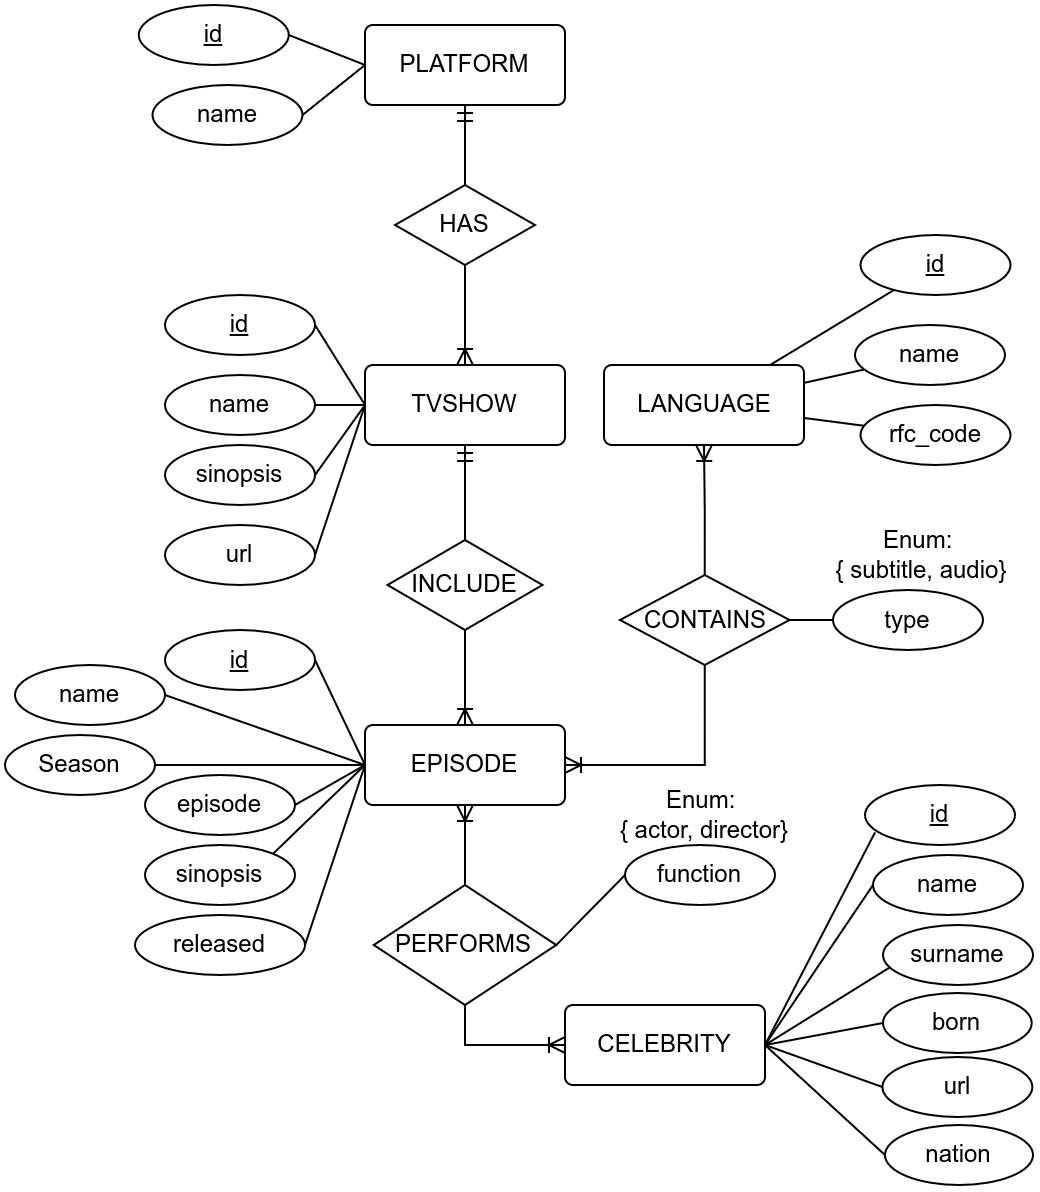
\includegraphics[width=0.8\linewidth]{img/entidad-relacion.png}
\end{center}


Este esquema entidad-relación ha dado lugar a un total de siete tablas cuyo esquema físico se puede importar tal como veremos más adelante.

\chapter{Despliegue de la aplicación}
Antes de entrar en detalle en cómo se ha desarrollado la aplicación es importante conocer cómo podemos realizar el despliegue de la aplicación, ya sea para utilizarla o para realizar modificaciones sobre la misma.

\section{Servicios Docker}
Para realizar el desarrollo del proyecto se ha utilizado servicios a través de contenedores \textbf{\href{https://www.docker.com/}{Docker}}, los cuáles pueden ser levantados gracias al fichero \configfile{compose.yaml} y el comando \commandbox{docker-compose up}

Al levantar los servicios con el comando \textbf{docker-compose up} se hará uso de los siguientes puertos:
\vspace{-1em}
\begin{itemize}
    \item \textbf{80}: Para el entorno web, usando Nginx como servidor web.
    \item \textbf{3306}: Para la base de datos.
    \item \textbf{3307}: Para el acceso web a phpmyadmin.
\end{itemize}
\vspace{-1em}

Para el correcto funcionamiento del contenedor se hace uso del fichero \configfile{vhost.conf} que modifica la configuración del servicio Nginx para que funcione de manera correcta con Laravel.

\section{Despliegue del código fuente}
Para realizar el despliegue del código fuente sobre el contenedor del servicio web, el directorio \configdir{viudb} debe estar situado a la misma altura del fichero \configfile{compose.yaml}.

De esta manera, a la hora de levantar el servicio se crea un volumen compartiendo el directorio local \configdir{viudb} con otro dentro del contenedor, en la ruta \configdir{/app}, que es de donde se nutre Nginx.


\section{Creación de la base de datos}

El servicio de MySQL se encarga de crear una base de datos llamada \textbf{actividad2} en el momento en el que el servicio se levanta. También crea los siguientes credenciales de acceso a dicha base de datos:

\vspace{-1em}
\begin{itemize}
    \item usuario:  \textbf{actividad2}
    \item contraseña:  \textbf{4ct1v1d4d2}
\end{itemize}
\vspace{-1em}

\section{Despliegue de datos}
Para realizar el despliegue de datos, se va a utilizar dos características que tiene Laravel y que tienen que ver con el despliegue en la base de datos:

\vspace{-1em}
\begin{itemize}
    \item \textbf{Migrate}: Es una forma de tener un sistema de control de versiones del esquema de base de datos. De esta manera, se puede hacer evolucionar el esquema (tablas, columnas, índices, ...) a lo largo del tiempo y también volver a un punto anterior del mismo.
    \item \textbf{Seeds}: También conocido como “semillas”, nos posibilita añadir datos a las tablas que hemos creado. Normalmente se utiliza para crear datos al inicio del proyecto con datos que deben existir (o también datos de pruebas) para que se pueda utilizar el proyecto.
\end{itemize}
\vspace{-1em}

Para realizar el despliegue debemos conectarnos al contenedor donde tenemos el proyecto y lanzar los comandos que realizan el “migrate” y crean los datos. A continuación aparecen los comandos:

\begin{mycode}{Acceder al contenedor Docker para hacer el despliegue}{console}{}
#nos conectamos al contenedor
ruben@vega:~$ docker exec -it   actividad_2_php_1 /bin/bash

#vamos al directorio donde está el desarrollo
root@a7913ac7b97a:/# cd /app

#lanzamos el migrate
root@a7913ac7b97a:/app# php artisan migrate
Migration table created successfully.
Migrating: 2014_10_12_000000_create_users_table
...

#lanzamos el seed
root@a7913ac7b97a:/app# php artisan db:seed
Seeding: UserSeeder
Seeded:  UserSeeder (0.06 seconds)
...
\end{mycode}



\chapter{Desarrollo realizado}

Una vez tenemos realizado el despliegue, se va a profundizar en el desarrollo realizado, destacando los siguientes aspectos:

\section{Configuración de la aplicación}
Otro de los aspectos en los que Laravel nos facilita el desarrollo es en la creación de un fichero de que podemos utilizar para realizar la configuración de la aplicación: \configfile{.env}.

Este fichero se crea con configuración que se debe modificar para la gestión de distintas configuraciones, y lo hemos utilizado para:
\vspace{-1em}
\begin{itemize}
    \item \textbf{Acceso a base de datos}: Para configurar el acceso a base de datos tenemos las opciones: servidor, puerto, usuario, contraseña y nombre de la base de datos. \textbf{Estas opciones deben ser configuradas para el servidor correspondiente}.
    \item \textbf{Paginación}: Para configurar el número de items por página que se van a visualizar. Opción “VIEW\_PAGINATE”.
    \item Las distintas \textbf{opciones que un celebrity} puede participar en un episodio. Dado que en la base de datos lo hemos añadido como “enum”, lo hemos configurado como “CELEBRITY\_EPISODE\_FUNCTIONS”.
    \item Similar al caso anterior, pero para los \textbf{idiomas y los episodios} en la variable “LANGUAGE\_EPISODE\_TYPES”.
\end{itemize}
\vspace{-1em}

\section{Relación entre modelos}
A la hora de crear la base de datos se ha tenido en cuenta ciertas relaciones en los datos, y por ello los modelos también se tienen que relacionar entre sí.

Laravel nos permite crear dicha relación a través de los modelos, en donde se indica si un modelo pertenece a otro, o si tiene varios elementos de otro modelo.

Vamos a poner como ejemplo el modelo de los episodios, que pertenece a una serie, y a su vez contiene varias celebrities:

\begin{mycode}{Parte del modelo “Episode”}{javascript}{}
// devuelve la serie a la que pertenece
public function tvshow(){
    return $this->belongsTo('App\TVShow');
}

// devuelve las celebrities que tiene el capítulo a través de
// la tabla celebrity_episode
// hay que indicar la columna extra que tiene la tabla.
public function celebrities() {
    return $this->belongsToMany('App\Celebrity')
                    ->withPivot(['perform_as']);
}
\end{mycode}

De esta manera, a través de un episodio podremos obtener a qué serie pertenece y qué \textit{celebrities} aparecen en ese episodio y qué función realizan en el mismo.


\section{Validación de datos en formularios}
A la hora de introducir o actualizar datos es importante que exista una validación previa, para que así no llegue el error hasta la base de datos.

A lo largo del proyecto, para todos los modelos, se ha realizado la validación en todos los formularios en donde se ha tenido en cuenta alguna (o varias) de las siguientes validaciones, entre otras:

\vspace{-1em}
\begin{itemize}
    \item Existencia de datos en un campo.
    \item Número mínimo de caracteres introducidos.
    \item No duplicidad en alguno de los campos.
\end{itemize}
\vspace{-1em}

\begin{center}
    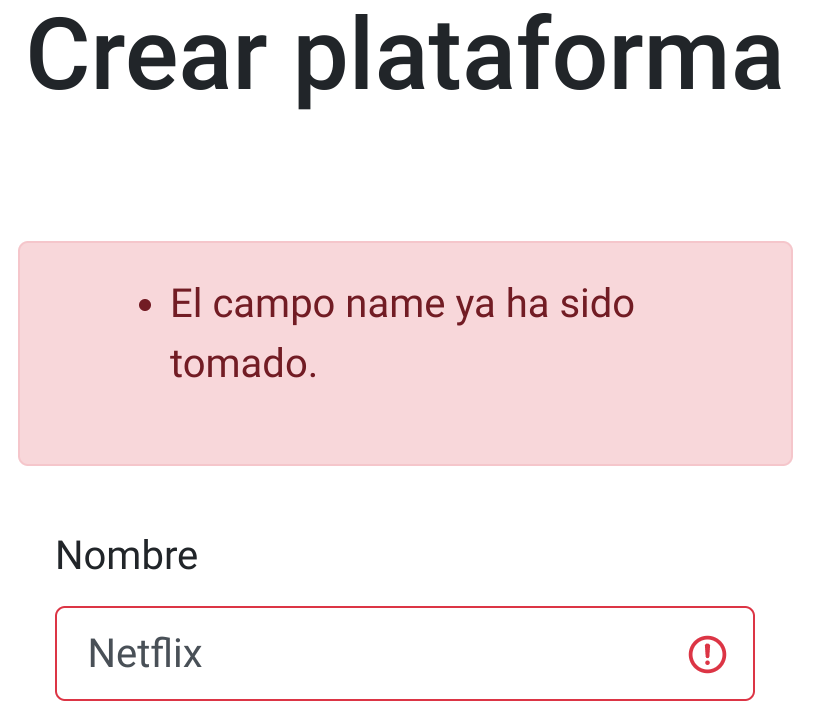
\includegraphics[frame,width=0.5\linewidth]{img/validacion.png}
\end{center}

En caso de que la validación de error, se vuelve al formulario y aparecerá el error y el campo del formulario que debe ser corregido, tal como aparece en la imagen.

\section{Autenticación y autorización}
Como parte del proyecto, era necesario crear un sistema de autenticación y autorización.

\vspace{-1em}
\begin{itemize}
    \item \textbf{Autenticación}: Proceso que se encarga de confirmar que un usuario es quien dice ser. Normalmente se valida con un usuario o e-mail y contraseña.
    \item \textbf{Autorización}: Proceso que permite a un usuario autenticado visitar, visualizar o utilizar ciertos recursos del proyecto.
\end{itemize}
\vspace{-1em}

\begin{center}
    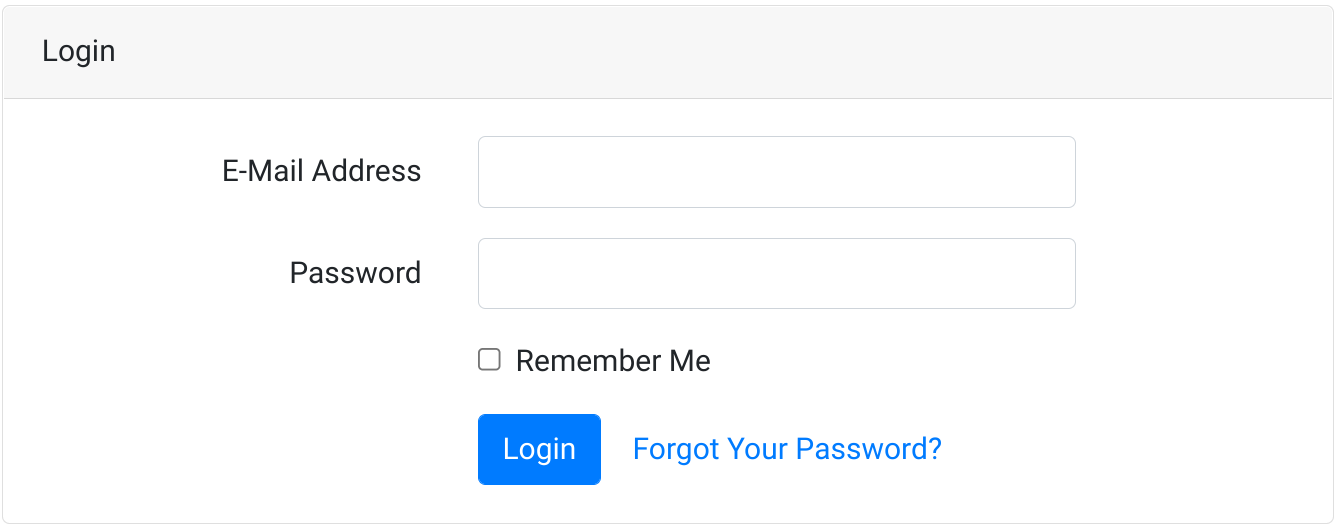
\includegraphics[width=0.5\linewidth]{img/login.png}
\end{center}

En este proyecto sólo el apartado de “plataformas” es público, por lo que para poder utilizar cualquier otro es necesario haberse autenticado. Usando el sistema de despliegue de datos se ha añadido un usuario para poder acceder todos a los apartados, siendo los credenciales:

\vspace{-1em}
\begin{itemize}
    \item \textbf{e-mail}: example@example.com
    \item \textbf{Password}: password
\end{itemize}
\vspace{-1em}



\section{Localización del proyecto}
Se denomina “localización” (o internacionalización) al diseño de software que tiene en cuenta que el proyecto realizado será utilizado en distintos idiomas. Este diseño permite que la traducción a otros idiomas que no sea el original sea más sencillo de realizar y que mediante una directiva de configuración se pueda cambiar.

\begin{center}
    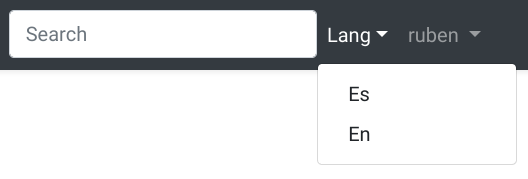
\includegraphics[width=0.5\linewidth]{img/languages.png}
\end{center}

En la barra de navegación, junto al sistema de búsqueda y de acceso se ha añadido un menú desplegable con los dos idiomas que se pueden utilizar actualmente en el desarrollo.


\section{Búsqueda de datos}

Para facilitar el acceso de los datos por parte de los usuarios se han añadido distintas cajas de búsqueda:

\vspace{-1em}
\begin{itemize}
    \item \textbf{Búsqueda general}: Se encuentra en la barra de navegación superior, para realizar una búsqueda entre todos los datos guardados de la aplicación
    \item \textbf{Búsqueda simple}: Dentro de cada apartado de la web hay otro buscador, pero este sólo busca en dicho apartado.
\end{itemize}
\vspace{-1em}

\begin{center}
    
\includegraphics[frame,width=0.5\linewidth]{img/buscar.png}
\end{center}

Si se usa el buscador general los resultados de búsqueda nos llevará a una página en la que aparecerán los resultados de la misma, resaltando el término buscado, tal como aparece en la imagen.


\chapter{Dificultades del proyecto}

Teniendo en cuenta que este proyecto es la continuación de uno anterior, se puede determinar que se han subsanado ciertas dificultadas expuestas en el anterior proyecto.

Ahora bien, eso no quita que hayan existido otras, que se exponen a continuación:

\vspace{-1em}
\begin{itemize}
    \item \textbf{Desconocimiento al usar el \textit{framework}}: A la hora de hacer uso de un \textit{framework} hay que conocer sus particularidades, pero bien es cierto que al haber usado otros (como Ruby on Rails), la curva de aprendizaje es menor. Aunque bien es cierto que el proceso de adaptación, conocer dónde se sitúan los ficheros, ver cómo se traspasa el conocimiento que se tiene de uno a otro, ... lleva su tiempo.
    \item \textbf{Falta de utilidades}: Teniendo en cuenta el punto anterior, se han echado de menos utilidades que otros frameworks incorporan de manera automática, como es el sistema de \textit{\textbf{scaffolding}} que genere: creación del \textit{migrate} pudiendo pasar los campos por línea de comandos; vistas CRUD para los modelos de datos; funciones CRUD que puedan ser utilizadas (no que están vacías)... Algunos de estos aspectos no se entienden ya que otros frameworks los tienen implementados desde el año 2006, por lo que es fácil coger esas ideas.
    \item \textbf{Uso de las validaciones}: El crear el sistema de validación teniendo en cuenta que no se repitan varios campos no es demasiado intuitivo, y en la documentación oficial no aparece rastro de ello.
\end{itemize}
\vspace{-1em}


\chapter{Conclusiones}

A la hora de desarrollar una aplicación web es importante conocer cómo se gestiona la información en el lado de servidor. Este proyecto ha permitido profundizar en diferentes ámbitos utilizados en el desarrollo \textbf{back-end} como son: el patrón \textbf{MVC}, la validación de datos obtenidos en peticiones, la creación de una aplicación multi-idioma, ...

El uso de Laravel como framework ha facilitado la labor de crear el proyecto en un tiempo ajustado, gracias a las implementaciones propias que tiene, lo que hace que también haya surgido un interés en comprobar las novedades que tienen las últimas versiones, y hacer un seguimiento del mismo.

\end{document}
